\documentclass[tikz,border=10pt]{standalone}
\usepackage{tikz}
\usetikzlibrary{shapes,arrows,positioning,shadows,fit}

\begin{document}

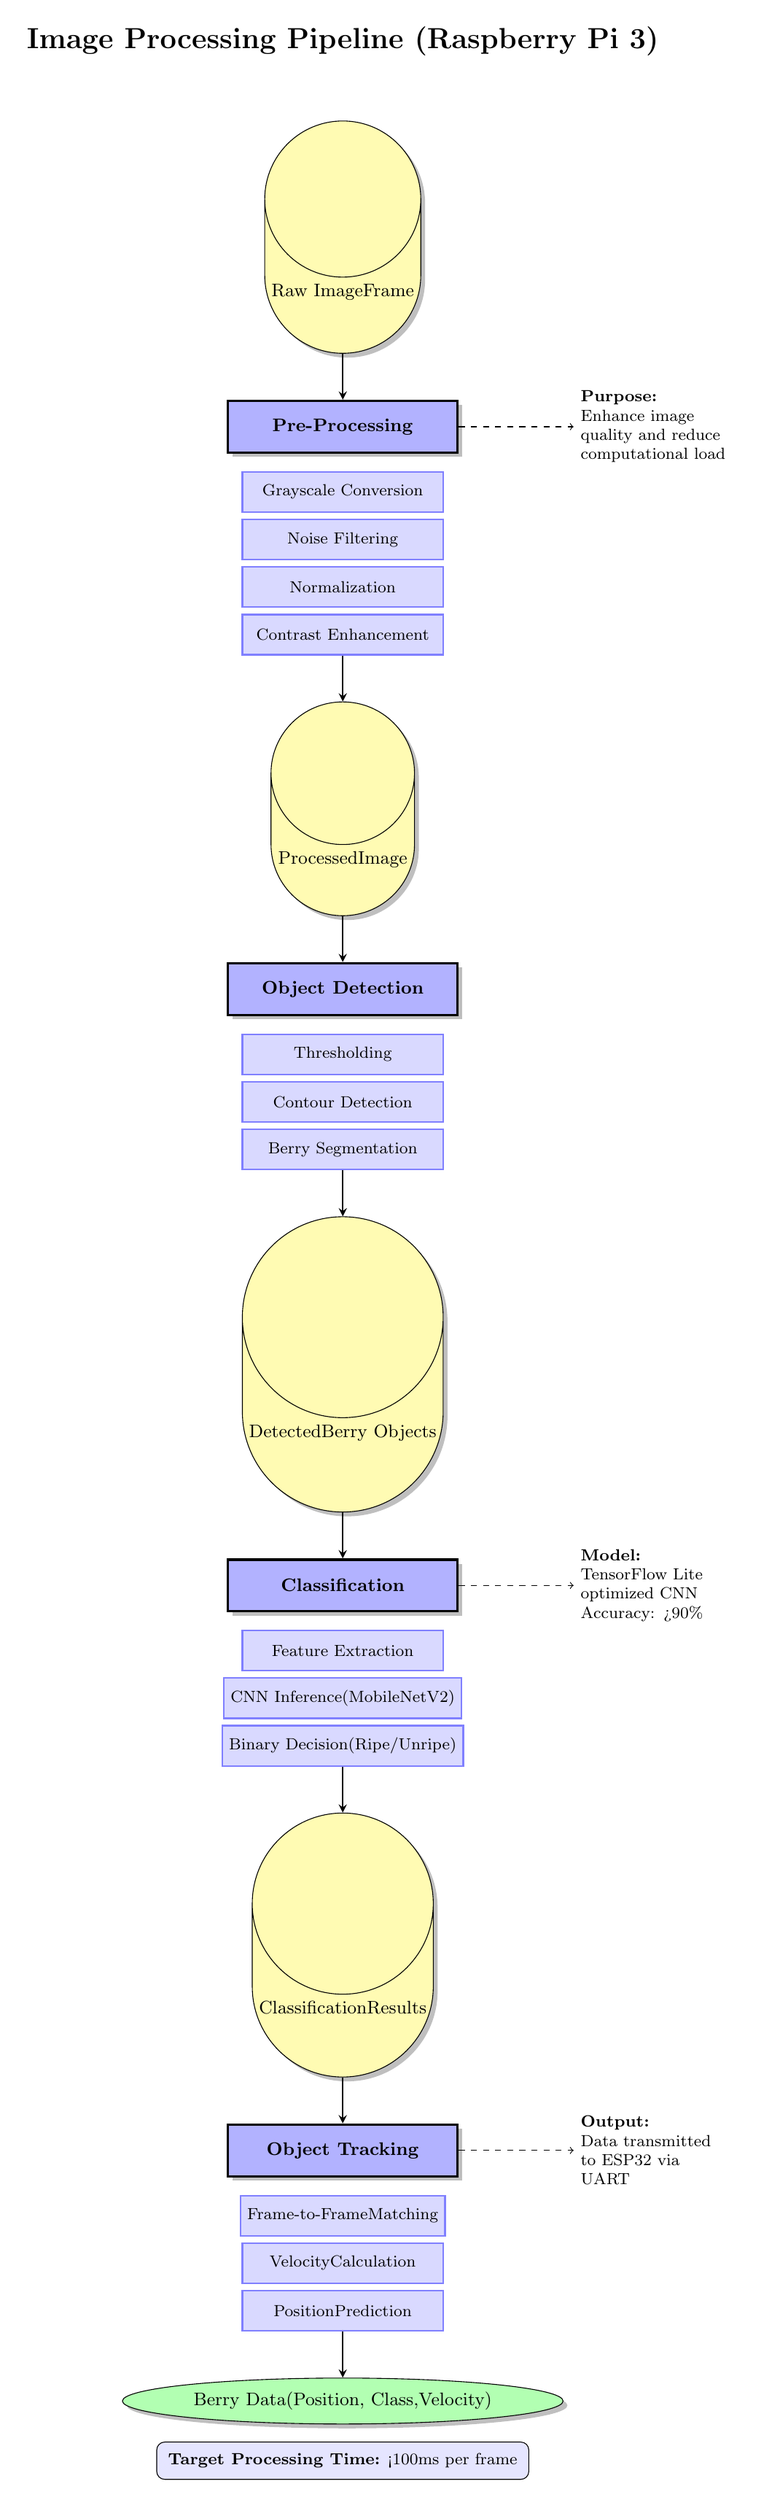
\begin{tikzpicture}[
    node distance=0.8cm,
    process/.style={rectangle, minimum width=4cm, minimum height=0.9cm, text centered, draw=black, fill=blue!30, drop shadow, very thick, font=\small},
    subprocess/.style={rectangle, minimum width=3.5cm, minimum height=0.7cm, text centered, draw=blue!50, fill=blue!15, thick, font=\footnotesize},
    data/.style={cylinder, shape border rotate=90, minimum width=2.5cm, minimum height=0.8cm, text centered, draw=black, fill=yellow!30, drop shadow, font=\small},
    result/.style={ellipse, minimum width=2.5cm, minimum height=0.8cm, text centered, draw=black, fill=green!30, drop shadow, font=\small},
    arrow/.style={thick,->,>=stealth},
    title/.style={font=\bfseries\Large}
]

% Title
\node[title] (title) {Image Processing Pipeline (Raspberry Pi 3)};

% Raw image input
\node[data, below=1cm of title] (raw) {Raw Image\\Frame};

% Pre-processing stage
\node[process, below=of raw] (preproc) {\textbf{Pre-Processing}};
\node[subprocess, below=0.3cm of preproc] (gray) {Grayscale Conversion};
\node[subprocess, below=0.1cm of gray] (filter) {Noise Filtering};
\node[subprocess, below=0.1cm of filter] (norm) {Normalization};
\node[subprocess, below=0.1cm of norm] (contrast) {Contrast Enhancement};

% Processed image
\node[data, below=0.8cm of contrast] (procimg) {Processed\\Image};

% Detection stage
\node[process, below=of procimg] (detection) {\textbf{Object Detection}};
\node[subprocess, below=0.3cm of detection] (thresh) {Thresholding};
\node[subprocess, below=0.1cm of thresh] (contour) {Contour Detection};
\node[subprocess, below=0.1cm of contour] (segment) {Berry Segmentation};

% Detected objects
\node[data, below=0.8cm of segment] (objects) {Detected\\Berry Objects};

% Classification stage
\node[process, below=of objects] (class) {\textbf{Classification}};
\node[subprocess, below=0.3cm of class] (extract) {Feature Extraction};
\node[subprocess, below=0.1cm of extract] (cnn) {CNN Inference\\(MobileNetV2)};
\node[subprocess, below=0.1cm of cnn] (decision) {Binary Decision\\(Ripe/Unripe)};

% Classification result
\node[data, below=0.8cm of decision] (classresult) {Classification\\Results};

% Tracking stage
\node[process, below=of classresult] (tracking) {\textbf{Object Tracking}};
\node[subprocess, below=0.3cm of tracking] (match) {Frame-to-Frame\\Matching};
\node[subprocess, below=0.1cm of match] (velocity) {Velocity\\Calculation};
\node[subprocess, below=0.1cm of velocity] (position) {Position\\Prediction};

% Final output
\node[result, below=0.8cm of position] (output) {Berry Data\\(Position, Class,\\Velocity)};

% Arrows
\draw[arrow] (raw) -- (preproc);
\draw[arrow] (contrast) -- (procimg);
\draw[arrow] (procimg) -- (detection);
\draw[arrow] (segment) -- (objects);
\draw[arrow] (objects) -- (class);
\draw[arrow] (decision) -- (classresult);
\draw[arrow] (classresult) -- (tracking);
\draw[arrow] (position) -- (output);

% Side annotations
\node[right=2cm of preproc, text width=3cm, font=\footnotesize, align=left] (note1) {
    \textbf{Purpose:}\\
    Enhance image\\quality and reduce\\computational load
};
\draw[->, dashed] (preproc) -- (note1);

\node[right=2cm of class, text width=3cm, font=\footnotesize, align=left] (note2) {
    \textbf{Model:}\\
    TensorFlow Lite\\optimized CNN\\Accuracy: >90\%
};
\draw[->, dashed] (class) -- (note2);

\node[right=2cm of tracking, text width=3cm, font=\footnotesize, align=left] (note3) {
    \textbf{Output:}\\
    Data transmitted\\to ESP32 via\\UART
};
\draw[->, dashed] (tracking) -- (note3);

% Processing time indicator
\node[below=0.3cm of output, fill=blue!10, draw, rounded corners, inner sep=0.2cm, font=\footnotesize] (time) {
    \textbf{Target Processing Time:} <100ms per frame
};

\end{tikzpicture}

\end{document}
